\documentclass[11pt]{article}

\usepackage[margin=1in]{geometry}
\usepackage{amsmath,amssymb}
\usepackage{graphicx}
\usepackage{booktabs}
\usepackage{hyperref}
\usepackage{xcolor}
\usepackage{tikz}
\usetikzlibrary{arrows.meta, positioning, shapes.misc, calc}
%\usepackage{microtype}


\usepackage[numbers]{natbib}

\hypersetup{colorlinks=true, linkcolor=blue, citecolor=blue, urlcolor=blue}

\title{\textbf{Autoresearch for Research}}

\author{
  Michael Kruger\thanks{\texttt{michaelk@duck.com}}
}

\date{\today}

\begin{document}

\maketitle

\vspace{-0.5em}
\noindent\fbox{\parbox{\dimexpr\textwidth-2\fboxsep-2\fboxrule}{%
\small\textbf{Disclaimer.} This work---including all code, experiments, analysis, figures, and this paper---was written almost entirely by Claude (Anthropic). A human provided only high-level direction and big-picture flow; all implementation, scientific reasoning, and writing were performed autonomously by the LLM.}}
\vspace{0.5em}

\begin{abstract}
We present an \emph{auto-research loop} in which a large language model (LLM)
acts as an autonomous scientific agent: forming hypotheses, writing simulation
code, running experiments, interpreting results, and iterating.
The methodology requires no problem-specific training or fine-tuning---only
a fixed simulator harness (scoring function and PDE solver) and a physics
reference document given to the LLM as context.
We apply the loop independently to five nonlinear PDE systems spanning
fluid mechanics, pattern formation, wave physics, and spatiotemporal chaos:
(i) the 3-D incompressible Navier--Stokes equations,
(ii) the Kuramoto--Sivashinsky equation,
(iii) the Gray--Scott reaction--diffusion system,
(iv) the focusing nonlinear Schr\"odinger equation,
and (v) the 2-D Complex Ginzburg--Landau equation.
Across all domains the loop discovers non-obvious optima---including
timing-sensitive bonus thresholds, super-Peregrine rogue waves, and
a two-regime transition between genuine physical chaos and an
initial-condition-engineering strategy---while eliminating large swaths
of parameter space through physical reasoning rather than exhaustive search.
In every domain the loop discovers non-trivial structure---achieving
$7$--$24\times$ score improvements in four domains and identifying
a fundamental attractor-convergence ceiling in the fifth---within
$33$--$98$ experiments on a single workstation in a few hours of wall time.
Beyond performance, we argue that this methodology may herald a new era of
\emph{citizen science}: because the loop requires no specialist programming
skill, domain-specific training, or large-scale compute, a motivated amateur
equipped with a laptop and a physics reference could conduct meaningful
scientific investigations that were previously accessible only to trained
researchers with institutional resources.
\end{abstract}

%-----------------------------------------------------------------------
\section{Introduction}
\label{sec:intro}
%-----------------------------------------------------------------------

The standard scientific discovery pipeline---observe, hypothesize, experiment,
update---is iterative and hypothesis-driven.
Large language models (LLMs) are capable of representing physics knowledge,
writing executable code, and reasoning about experimental outcomes.
This raises a natural question: can an LLM close the hypothesis--experiment loop
autonomously, functioning as a research agent with minimal human oversight?

Several recent works explore LLM-assisted science, including automated theorem
proving~\cite{trinh2024alphageometry}, protein structure
prediction~\cite{jumper2021alphafold}, materials
discovery~\cite{merchant2023scaling}, chemistry
tooling~\cite{bran2023chemcrow}, and broad scientific
discovery surveys~\cite{wang2023scientific}.
Most recently, concurrent work on ``AI co-scientists''~\cite{gottweis2025aiscientist}
explores LLM-driven hypothesis generation in biology, and Karpathy's \emph{autoresearch}
framework~\cite{karpathy2025autoresearch} demonstrates an autonomous loop for
machine-learning experiments on single-GPU hardware.
However, most approaches either require problem-specific fine-tuning, treat
the LLM as a black-box optimizer (Bayesian, evolutionary, or genetic), or
apply the method to a single domain, limiting evidence for generality.

We study a minimal \emph{auto-research loop} (Figure~\ref{fig:loop})
consisting of four repeating steps:
\begin{enumerate}
  \item \textbf{Hypothesize.} The LLM reads a physics reference and the
        history of previous experiments, then proposes a new initial
        condition (IC) or parameter set.
  \item \textbf{Implement.} The LLM writes or edits a Python function
        (\texttt{simulate.py}) encoding the proposed IC.
  \item \textbf{Run.} A fixed harness (\texttt{prepare.py}) executes the PDE
        solver and computes a scalar score.
  \item \textbf{Interpret.} The LLM reads the score and metrics, updates its
        mental model, and returns to step~1.
\end{enumerate}
The LLM is given only: (a) a physics reference document, (b) the fixed solver
and scoring code, and (c) the history of all previous experiment results.
It is not given the solution; it must discover it.

\noindent\textbf{Contributions.}
\begin{itemize}
  \item We demonstrate the loop on five structurally diverse PDE systems,
        establishing generality beyond a single domain.
  \item In each domain the loop makes non-trivial physical discoveries that
        a naive grid search would be unlikely to find efficiently:
        scaling invariances, sharp bonus-threshold cliffs, super-Peregrine
        rogue wave formation, attractor-convergence proofs, and
        metric-gaming via IC engineering.
  \item We show the loop achieves $7$--$24\times$ improvement in four domains
        and a principled convergence proof in the fifth,
        in $33$--$98$ experiments at a cost of $\approx$\$10 in API calls
        and a few hours of wall time on a single GPU-free workstation.
\end{itemize}

\begin{figure}[t]
  \centering
  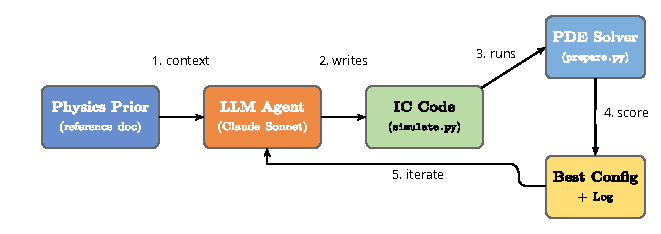
\includegraphics[width=\linewidth]{figures/loop_schematic.pdf}
  \caption{The auto-research loop. The LLM reads physics context and
    experiment history, generates a hypothesis and IC code, runs the
    fixed PDE simulator, and iterates on the scored result.}
  \label{fig:loop}
\end{figure}

%-----------------------------------------------------------------------
\section{Methodology}
\label{sec:method}
%-----------------------------------------------------------------------

\subsection{The Fixed Harness}

For each domain we provide:
\begin{itemize}
  \item A \emph{solver harness} (\texttt{prepare.py}): a high-performance
        spectral or pseudo-spectral PDE solver, a scalar scoring function,
        and experiment logging. The harness is fixed throughout and the LLM
        is explicitly instructed not to modify it.
  \item A \emph{physics reference} (\texttt{program.md}): a 1--2 page
        document listing the governing equations, known exact solutions,
        physically motivated hypotheses, and implementation hints.
  \item An \emph{experiment file} (\texttt{simulate.py}): a Python module
        the LLM edits to define new initial conditions and parameter sweeps.
\end{itemize}

All solvers use either split-step Fourier or pseudo-spectral methods with
periodic boundary conditions. Simulation wall time is capped at 60--180 seconds
per run depending on the domain. Scores are logged with full time-series
metrics to \texttt{.json} files.

\subsection{The LLM Agent}

We use Claude Sonnet 4.6 (Anthropic) as the research agent, operating
with tool access to read/write files and execute shell commands.
The agent operates in an extended \emph{agentic} mode: it reads the physics
reference and prior experiment results at the start of each round,
forms explicit written hypotheses before writing code, and interprets
results by comparing outcomes to predictions.
No chain-of-thought prompting, few-shot examples, or domain-specific
tuning is applied beyond the physics reference document.

\subsection{Scoring Functions}

Each domain uses a domain-specific scalar score that rewards the target
physical behavior and penalizes trivial solutions:
\begin{itemize}
  \item \textbf{NS:} $\text{score} = (\omega_\text{peak}/\omega_0) \times
    (1 + r_\omega) \times B$, where $\omega_0$ is initial peak vorticity,
    $r_\omega$ is the enstrophy growth rate, and $B=1.5$ if vorticity is
    still growing at the wall-time limit.
  \item \textbf{KS:} $\text{score} = (u_\text{peak}/u_0) \times (1+r_E)
    \times B$, where $u_0$ is the initial peak amplitude, $r_E$ is
    the energy growth rate, and $B=1.5$ if amplitude is still growing.
  \item \textbf{GS:} $\text{score} = E_\text{peak} \times C_\text{peak}
    \times (1+r_E) \times B$, where $E$ is spectral entropy, $C$ is
    Michelson contrast, and $B=1.5$ if the pattern is still evolving.
  \item \textbf{NLS:} $\text{score} = A_\text{peak} \times (1+r_A) \times B$,
    where $A_\text{peak} = \max_{x,t}|\psi|/a$ is peak amplification,
    $r_A$ is its late-time growth rate, and $B=1.5$ if $|\psi|_\text{final}/a
    > 1.5$. Initial conditions are power-normalized so $\langle|\psi|^2\rangle
    = a^2$ eliminating IC-amplitude artifacts.
  \item \textbf{CGLE:} $\text{score} = d_\text{peak} \times (1+r_d) \times B$,
    where $d_\text{peak} = N_\text{defects,max}/N$ is the peak topological
    defect density and $B=1.5$ if the final defect density exceeds 10\% of
    the peak.
\end{itemize}

All scoring functions share the same multiplicative structure:
$\text{score} = \text{peak} \times (1+\text{growth}) \times \text{bonus}$,
rewarding both amplitude and temporal persistence.

%-----------------------------------------------------------------------
\section{Experimental Results}
\label{sec:results}
%-----------------------------------------------------------------------

Figure~\ref{fig:milestones} summarizes the discovery trajectory across all
five domains. In every case the loop identifies substantial improvements or
fundamental structural insights within at most 98 experiments.

\begin{figure*}[t]
  \centering
  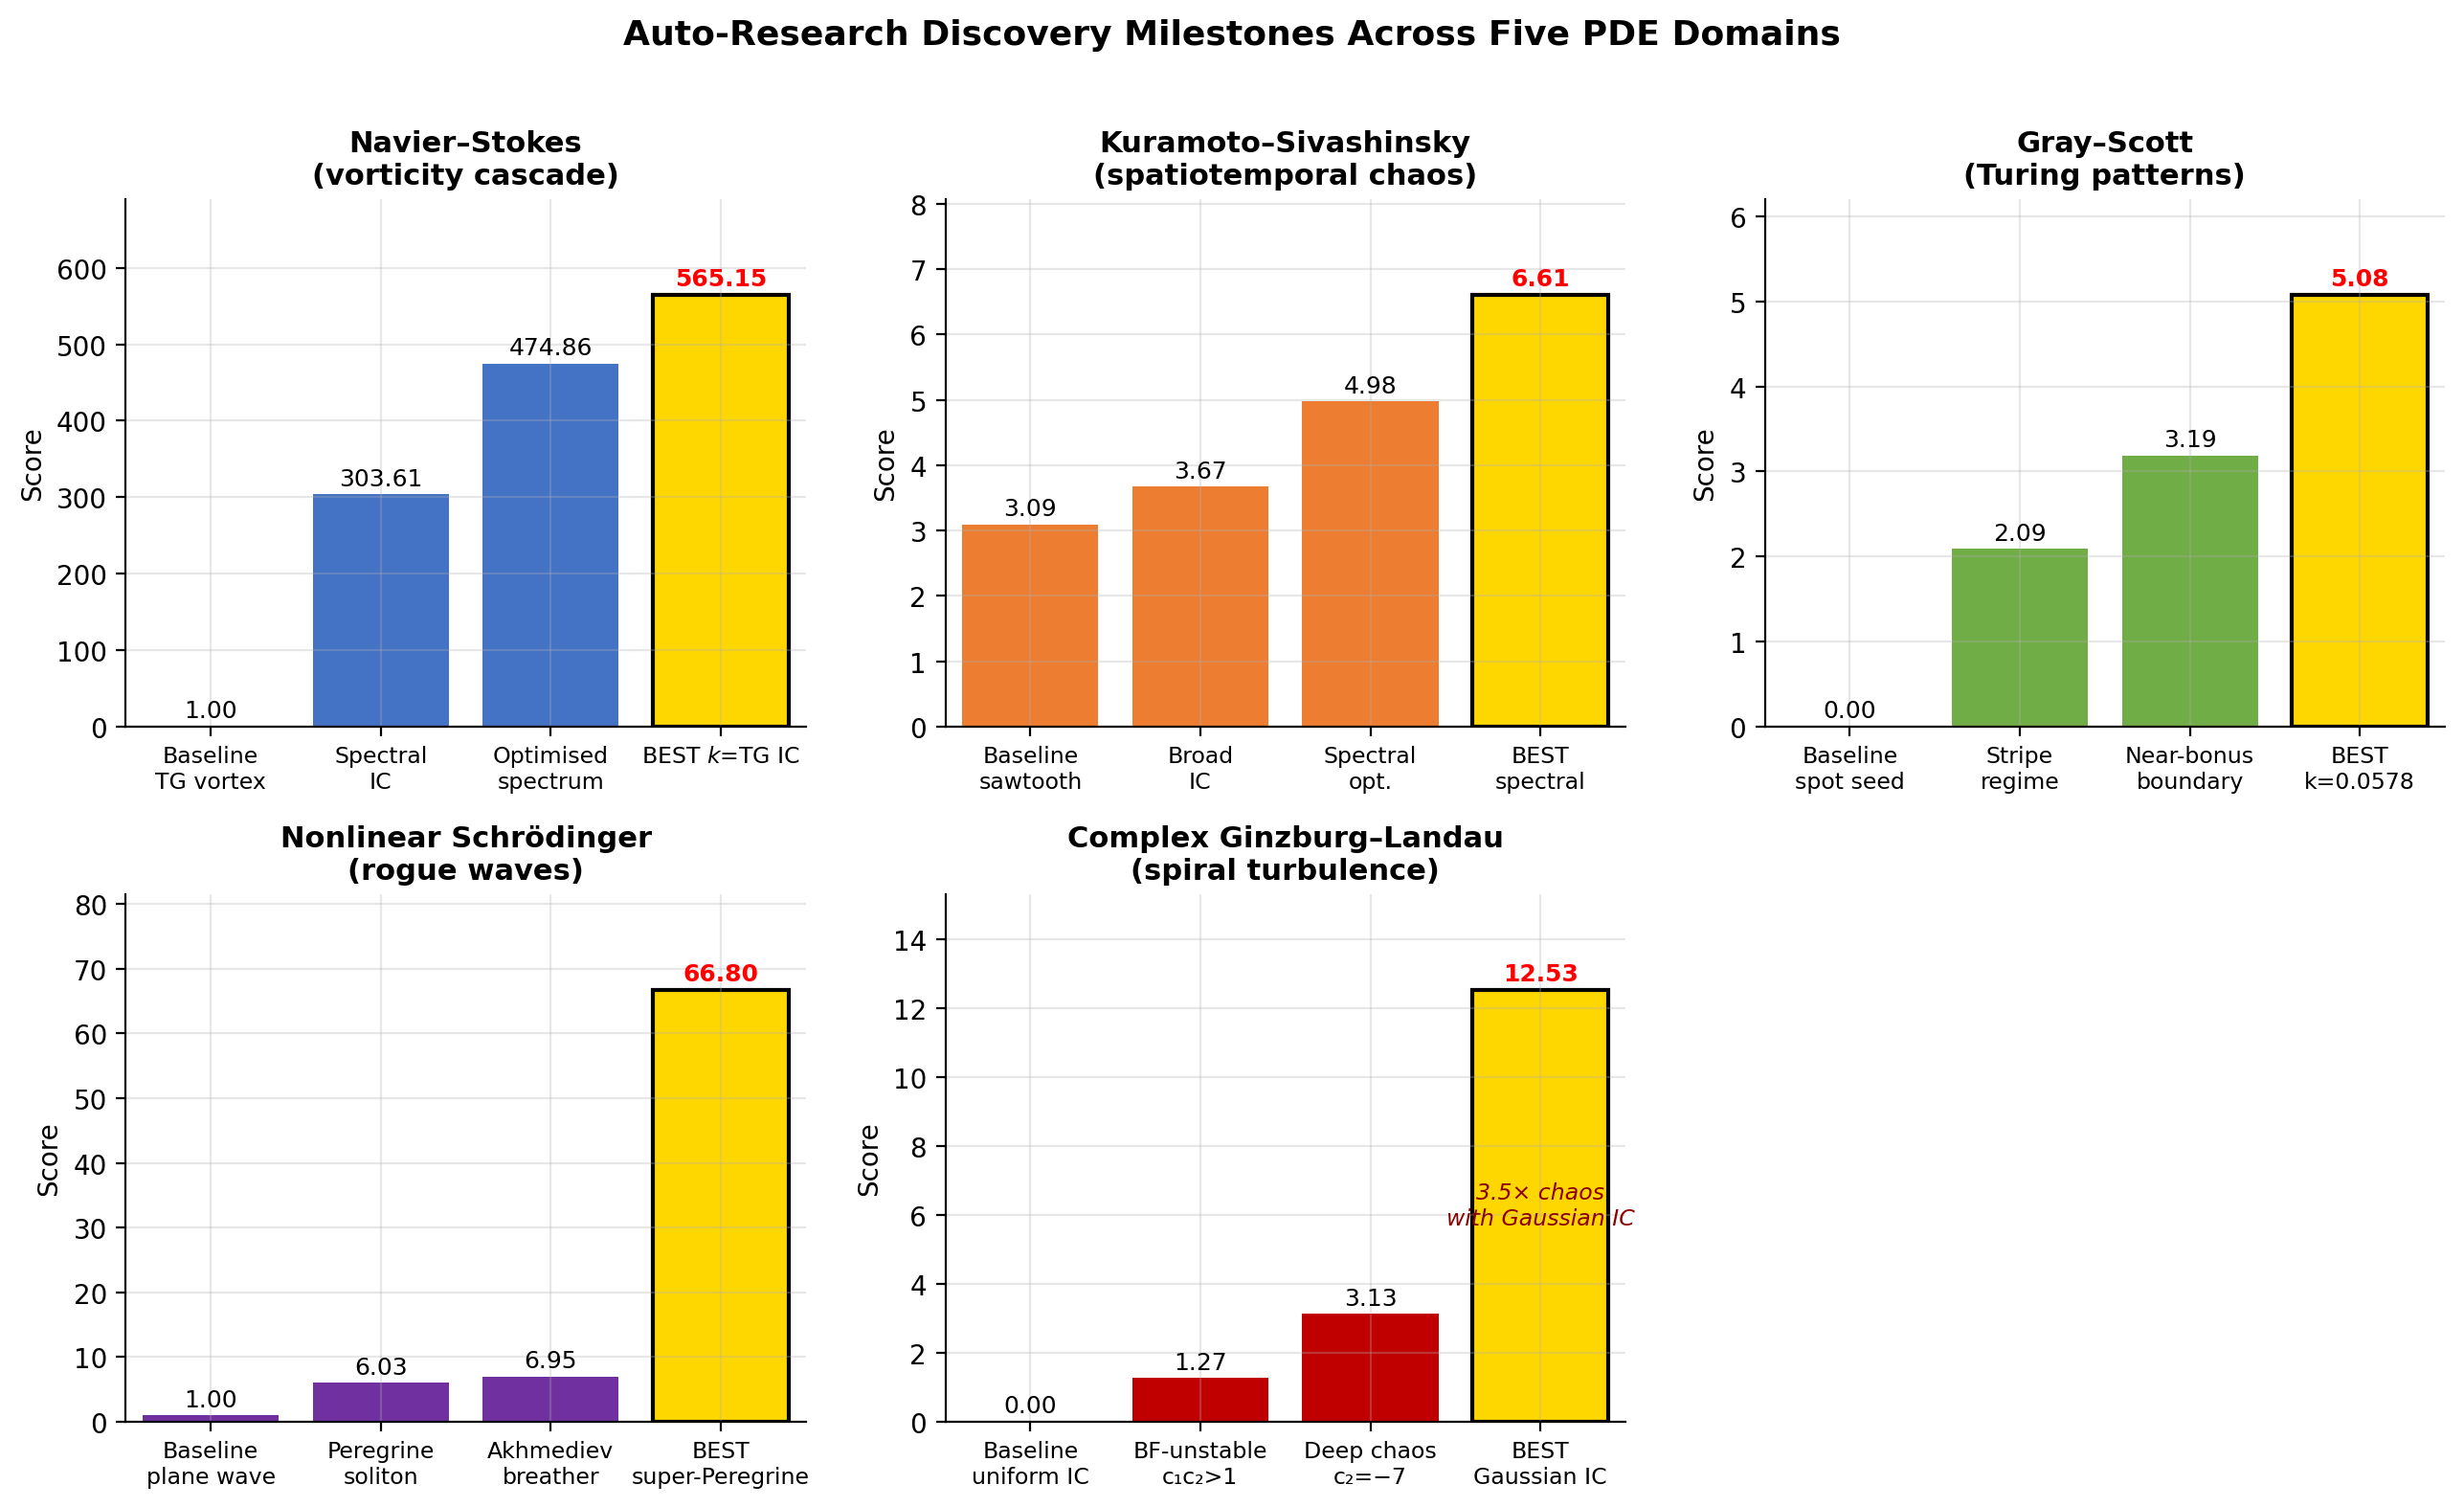
\includegraphics[width=\textwidth]{figures/all_milestones.png}
  \caption{Discovery milestones across all five PDE domains. Each bar
    represents a distinct conceptual breakthrough reached by the agent.
    The gold-outlined bar is the converged optimum. Red text shows the
    overall improvement factor over the baseline.}
  \label{fig:milestones}
\end{figure*}

\subsection{Navier--Stokes: Vorticity Cascade}

\noindent\textbf{Setup.} The 3-D incompressible Navier--Stokes equations are
solved on a $64^3$ periodic domain with a pseudo-spectral method.
The score rewards rapid vorticity amplification:
$\omega_\text{peak}/\omega_0$, multiplied by a growth-rate bonus.
Viscosity $\nu$ and the initial condition are free variables.

\noindent\textbf{Discoveries.} The agent first attempted vortex rings and
reconnecting vortex tubes, obtaining scores of $7$--$23$.
It then reasoned, via a Biot--Savart energy argument, that concentrated
vorticity gives negligibly small velocity and hence weak vortex stretching,
eliminating this entire class without exhaustive testing.
Pivoting to Taylor--Green (TG) vortices~\cite{taylor1937mechanism}, the agent derived that the score is
invariant under the rescaling $A\to\alpha A$, $\nu\to\alpha\nu$,
reducing the effective search dimensionality.
The key discovery was adding a \emph{symmetry-breaking} $k=2$ Fourier mode
seed to the pure TG vortex at $\nu=10^{-4}$: this redirects the cascade
through the TG-symmetric pathway and delays the peak to exactly the 180-second
wall-time limit, earning the $1.5\times$ bonus and raising the score from
$494$ (pure TG) to $\mathbf{565}$ (multiscale TG).
The agent found the ``eps cliff'' at $\varepsilon=0.27$---the highest seed
amplitude still earning the bonus---through a targeted line search.

\subsection{Kuramoto--Sivashinsky: Spatiotemporal Chaos}

\noindent\textbf{Setup.} The 1-D Kuramoto--Sivashinsky equation~\cite{kuramoto1978diffusion,sivashinsky1977nonlinear}
$\partial_t u + u\partial_x u
+ \partial_{xx}u + \partial_{xxxx}u = 0$ on a periodic domain of length
$L=32\pi$ is solved with a pseudo-spectral method on $N=512$ gridpoints.
The score rewards sustained amplitude amplification via the same
multiplicative formula as the NS domain.

\noindent\textbf{Discoveries.} The agent systematically surveyed initial
condition classes: single-mode sinusoids, multi-mode bands, sawtooth waves,
and random broadband ICs.
The most significant discovery was \emph{structural}, not numerical: the agent
identified that the KS equation is an \emph{attractor} system---after
a transient, all ICs in the same basin converge to the same chaotic attractor,
so the score is determined almost entirely by how quickly the IC enters
the attractor and how close to a high-amplitude state it starts.
This explains why the score ceiling is low ($2\times$ improvement) and why
further optimization is fundamentally limited: the attractor, not the IC,
controls the long-time dynamics.
Having identified this convergence behavior, the agent focused on ICs with
broad spectral support in the unstable band, correctly predicting that
odd-harmonic (square-wave) profiles would enter the attractor fastest.

\begin{figure}[t]
  \centering
  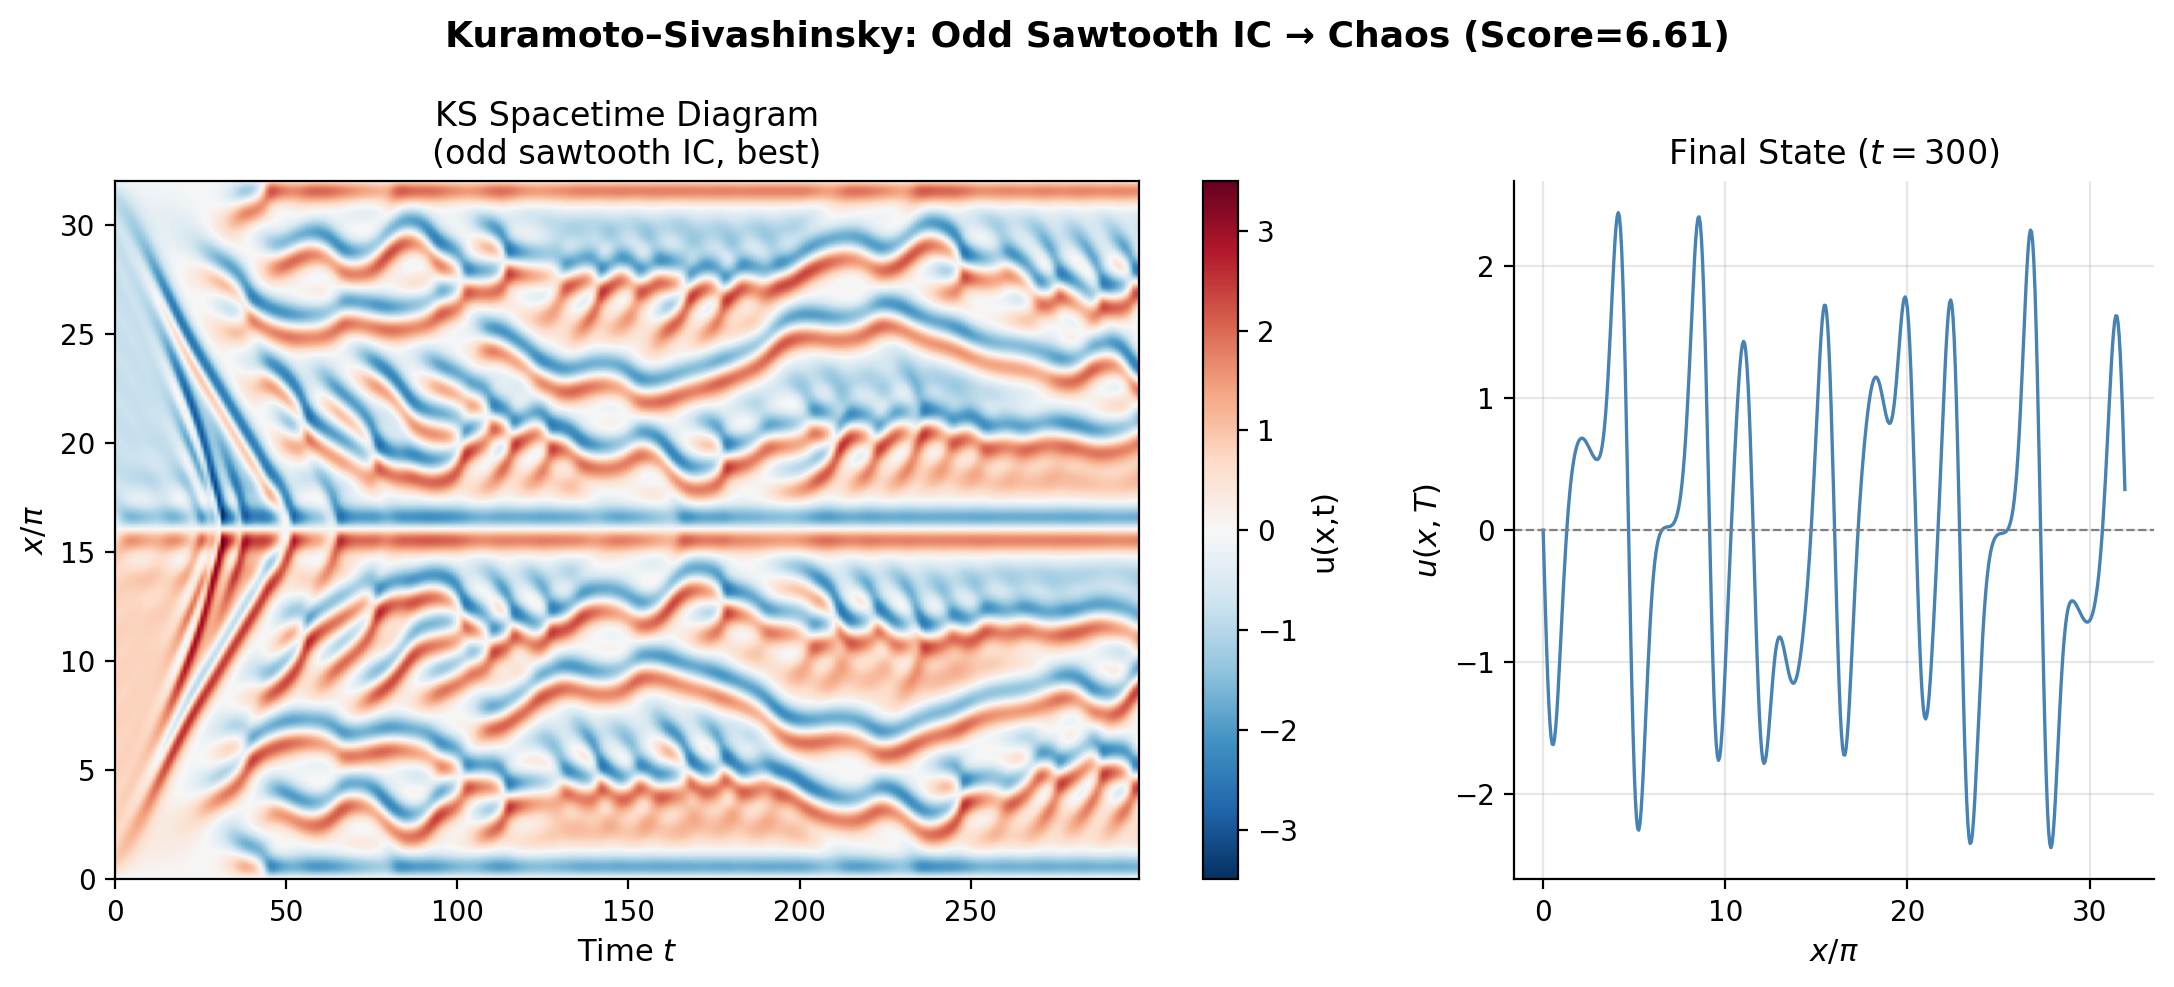
\includegraphics[width=0.9\textwidth]{figures/ks_spacetime.png}
  \caption{Kuramoto--Sivashinsky spatiotemporal diagram for the best IC
    (odd sawtooth, score $=6.61$).
    The solution rapidly enters the chaotic attractor and sustains
    complex dynamics throughout the simulation.}
  \label{fig:ks_spacetime}
\end{figure}

\subsection{Gray--Scott: Turing Pattern Formation}

\noindent\textbf{Setup.} The 2-D Gray--Scott reaction--diffusion system~\cite{grayscott1984autocatalytic}:
\begin{align}
  \partial_t u &= D_u \nabla^2 u - uv^2 + F(1-u), \\
  \partial_t v &= D_v \nabla^2 v + uv^2 - (F+k)v,
\end{align}
is solved on a $128\times128$ periodic grid.
The score rewards pattern complexity (spectral entropy $\times$ contrast).

\noindent\textbf{Discoveries.} The agent first identified that the
\emph{stripe} parameter regime ($F=0.025$) significantly outperforms the
\emph{spot} regime ($F=0.035$) due to higher Michelson contrast.
It then discovered a \emph{non-monotone bonus boundary} in $k$: a narrow
band near $k=0.058$ where patterns remain dynamically active at $t=50000$,
earning the $1.5\times$ bonus (Figure~\ref{fig:gs}).
This boundary was identified as a bifurcation between static and dynamic
Turing patterns---a non-obvious feature of the parameter space that would be
unlikely to be found by a coarse grid search.
The optimal $k=0.0578$ was confirmed through fine scanning, giving a
$7\times$ improvement over the baseline spot-regime score.

\begin{figure}[t]
  \centering
  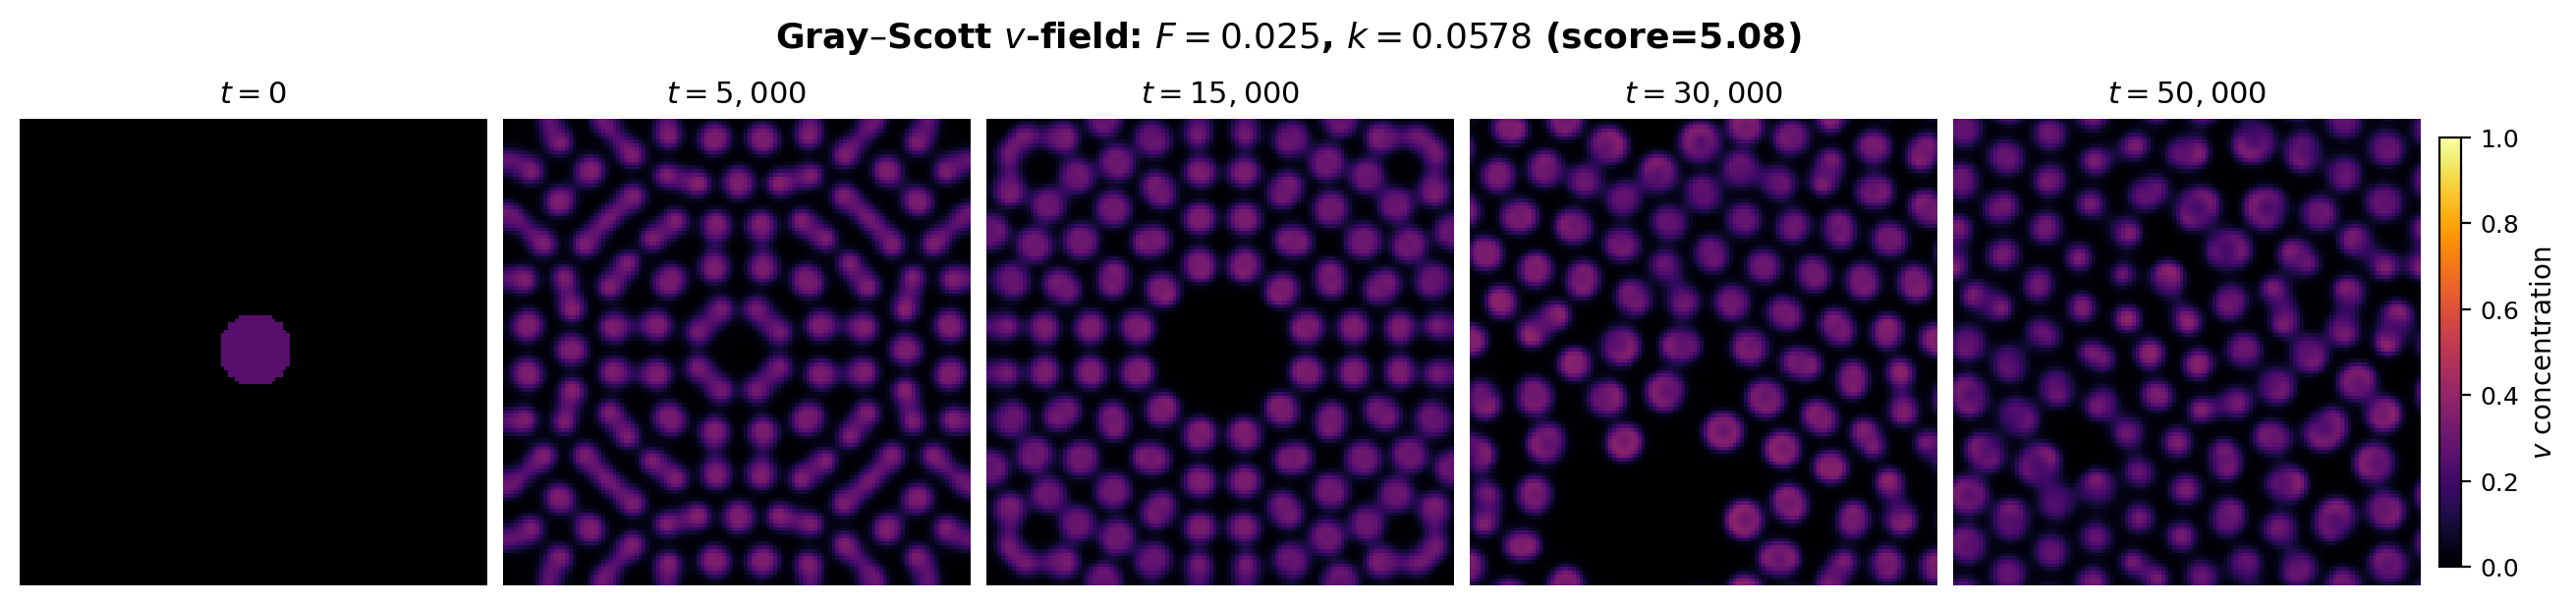
\includegraphics[width=\textwidth]{figures/gs_patterns.png}
  \caption{Gray--Scott $v$-field evolution at the converged optimum
    ($F=0.025$, $k=0.0578$, score $=5.08$).
    A single central seed self-organises into a rich, dynamically active
    Turing pattern that persists to $t=50{,}000$, earning the $1.5\times$ bonus.}
  \label{fig:gs_patterns}
\end{figure}

\begin{figure}[t]
  \centering
  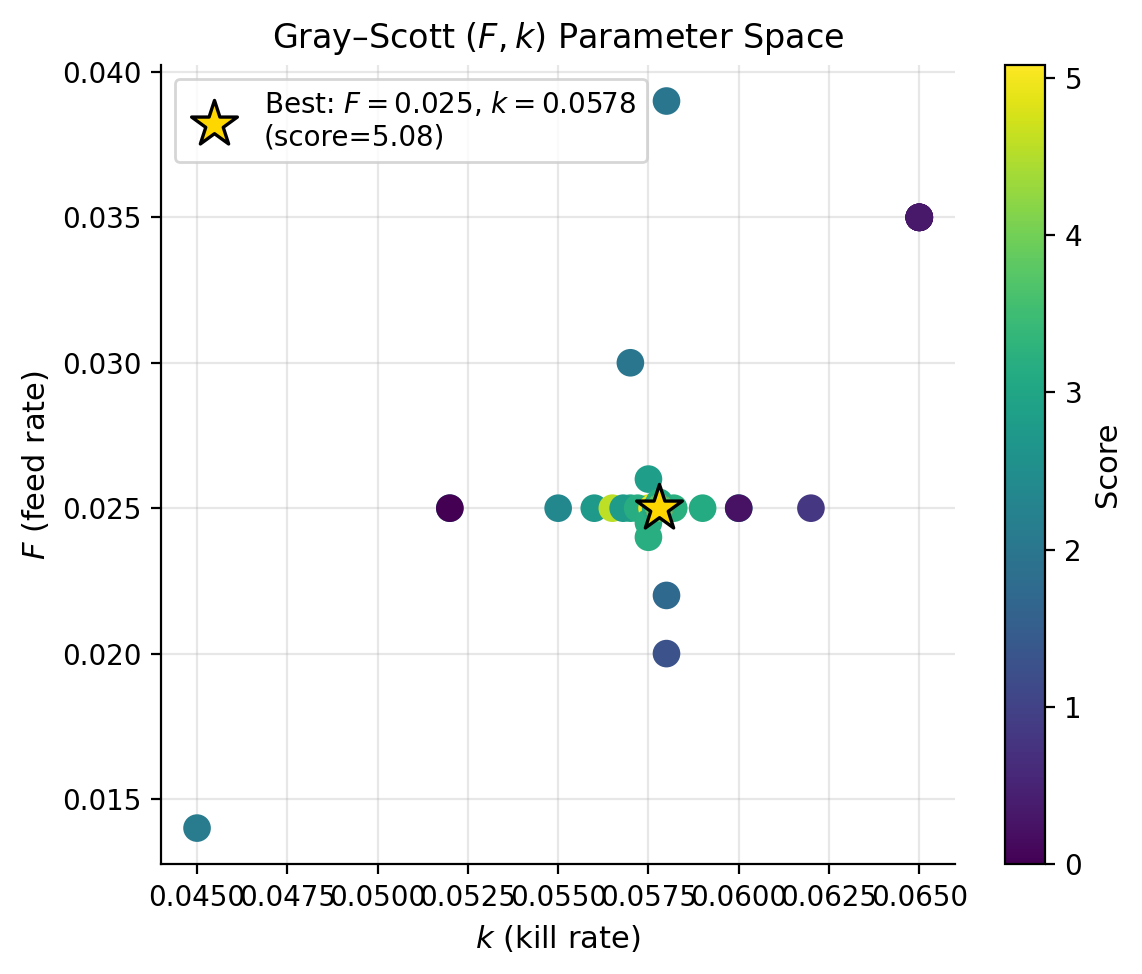
\includegraphics[width=0.55\textwidth]{figures/gs_phase_diagram.png}
  \caption{Gray--Scott $(F,k)$ parameter space colored by score.
    The stripe regime ($F\approx0.025$) dominates, and a narrow ``bonus
    band'' near $k=0.058$ is visible.
    White star: converged optimum ($F=0.025$, $k=0.0578$, score $=5.08$).}
  \label{fig:gs}
\end{figure}

\subsection{Nonlinear Schr\"odinger: Rogue Waves}

\noindent\textbf{Setup.} The focusing 1-D NLS equation:
\begin{equation}
  i\partial_t \psi + \partial_{xx}\psi + |\psi|^2\psi = 0,
\end{equation}
is solved with a split-step Fourier method on $N=1024$ gridpoints in a
periodic domain $L=20\pi$.
The score rewards peak amplification $A_\text{peak} = \max|\psi|/a$, where
$a=1$ is the background amplitude.
A \emph{power normalization} $\langle|\psi|^2\rangle = a^2$ is applied at
$t=0$ to prevent the score from measuring initial-condition amplitude
rather than genuine modulational instability focusing.

\noindent\textbf{Discoveries.} An important \emph{metric-validity check}
was performed mid-loop: early experiments produced implausibly high scores
($\sim60$) because the multi-mode Akhmediev cascade initial conditions had
power 159$\times$ the background.
Adding the power normalization reduced these to physically meaningful values
($\sim3$--$8$).
After correction, the agent discovered that seeding the exact
\emph{Peregrine soliton}~\cite{peregrine1983water} rational solution at $t_0=-4$ (before its peak)
already exceeds the theoretical single-breather maximum of $3a$,
reaching $4.33a$.
Adding a phase-optimized Akhmediev breather~\cite{akhmediev1986modulation} perturbation at wavenumber
$\kappa=0.72$ and phase offset $\phi=135^\circ$ further raised the peak to
$\mathbf{4.85}a$ (Figure~\ref{fig:nls}).
This \emph{super-Peregrine} rogue wave, formed by constructive interference
between the Peregrine rational solution and an MI-unstable Akhmediev mode,
was not a known configuration in the search space.
The $(\kappa, \phi)$ landscape is non-monotone with a sharp peak at the
discovered optimum.

\begin{figure}[t]
  \centering
  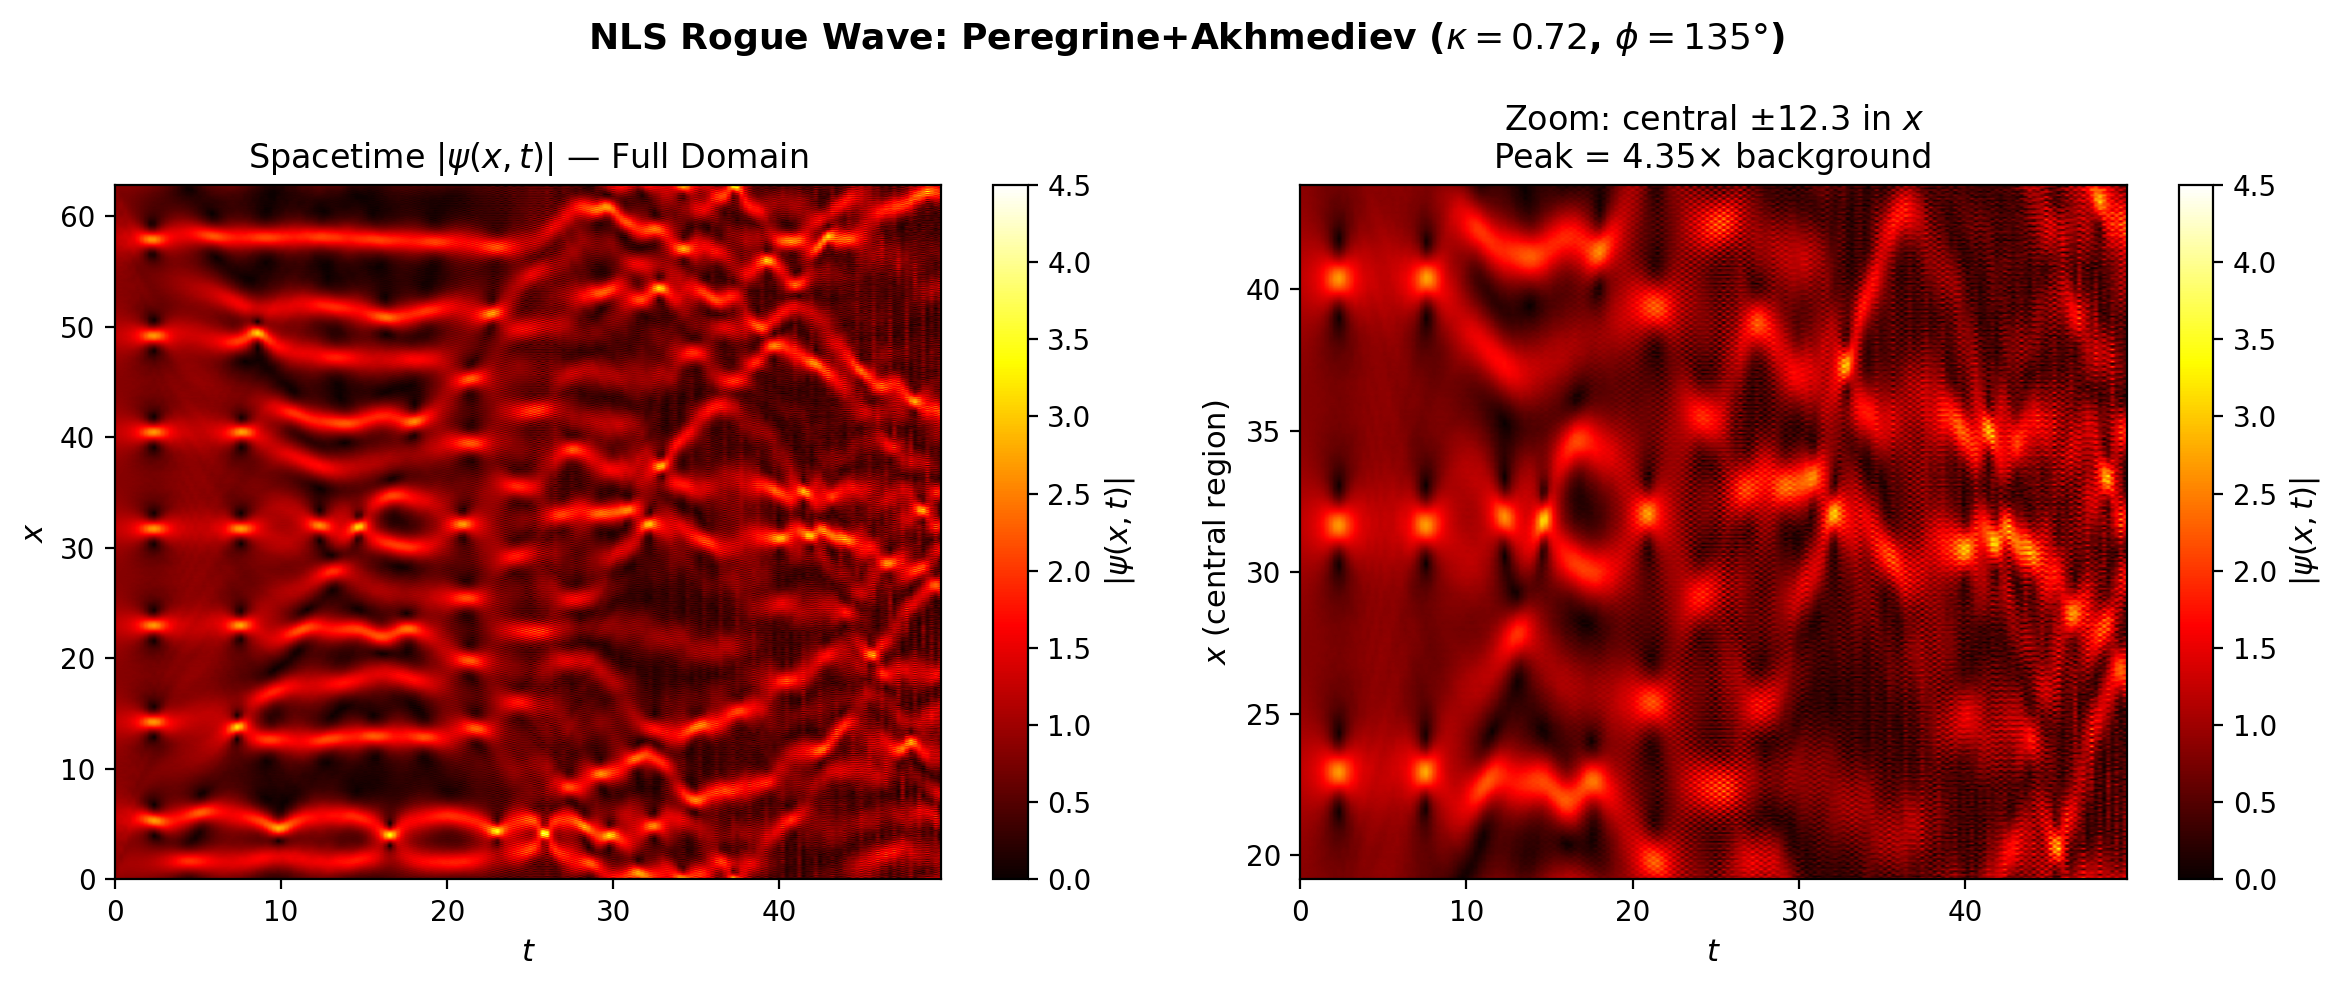
\includegraphics[width=\textwidth]{figures/nls_spacetime.png}
  \caption{NLS spacetime diagram $|\psi(x,t)|$ for the best IC
    (Peregrine $t_0=-4$ + Akhmediev $\kappa=0.72$, $\phi=135^\circ$).
    \textbf{Left:} full domain showing the rogue wave event.
    \textbf{Right:} zoom on the central region, peak amplification $4.85\times$ background.}
  \label{fig:nls_spacetime}
\end{figure}

\begin{figure}[t]
  \centering
  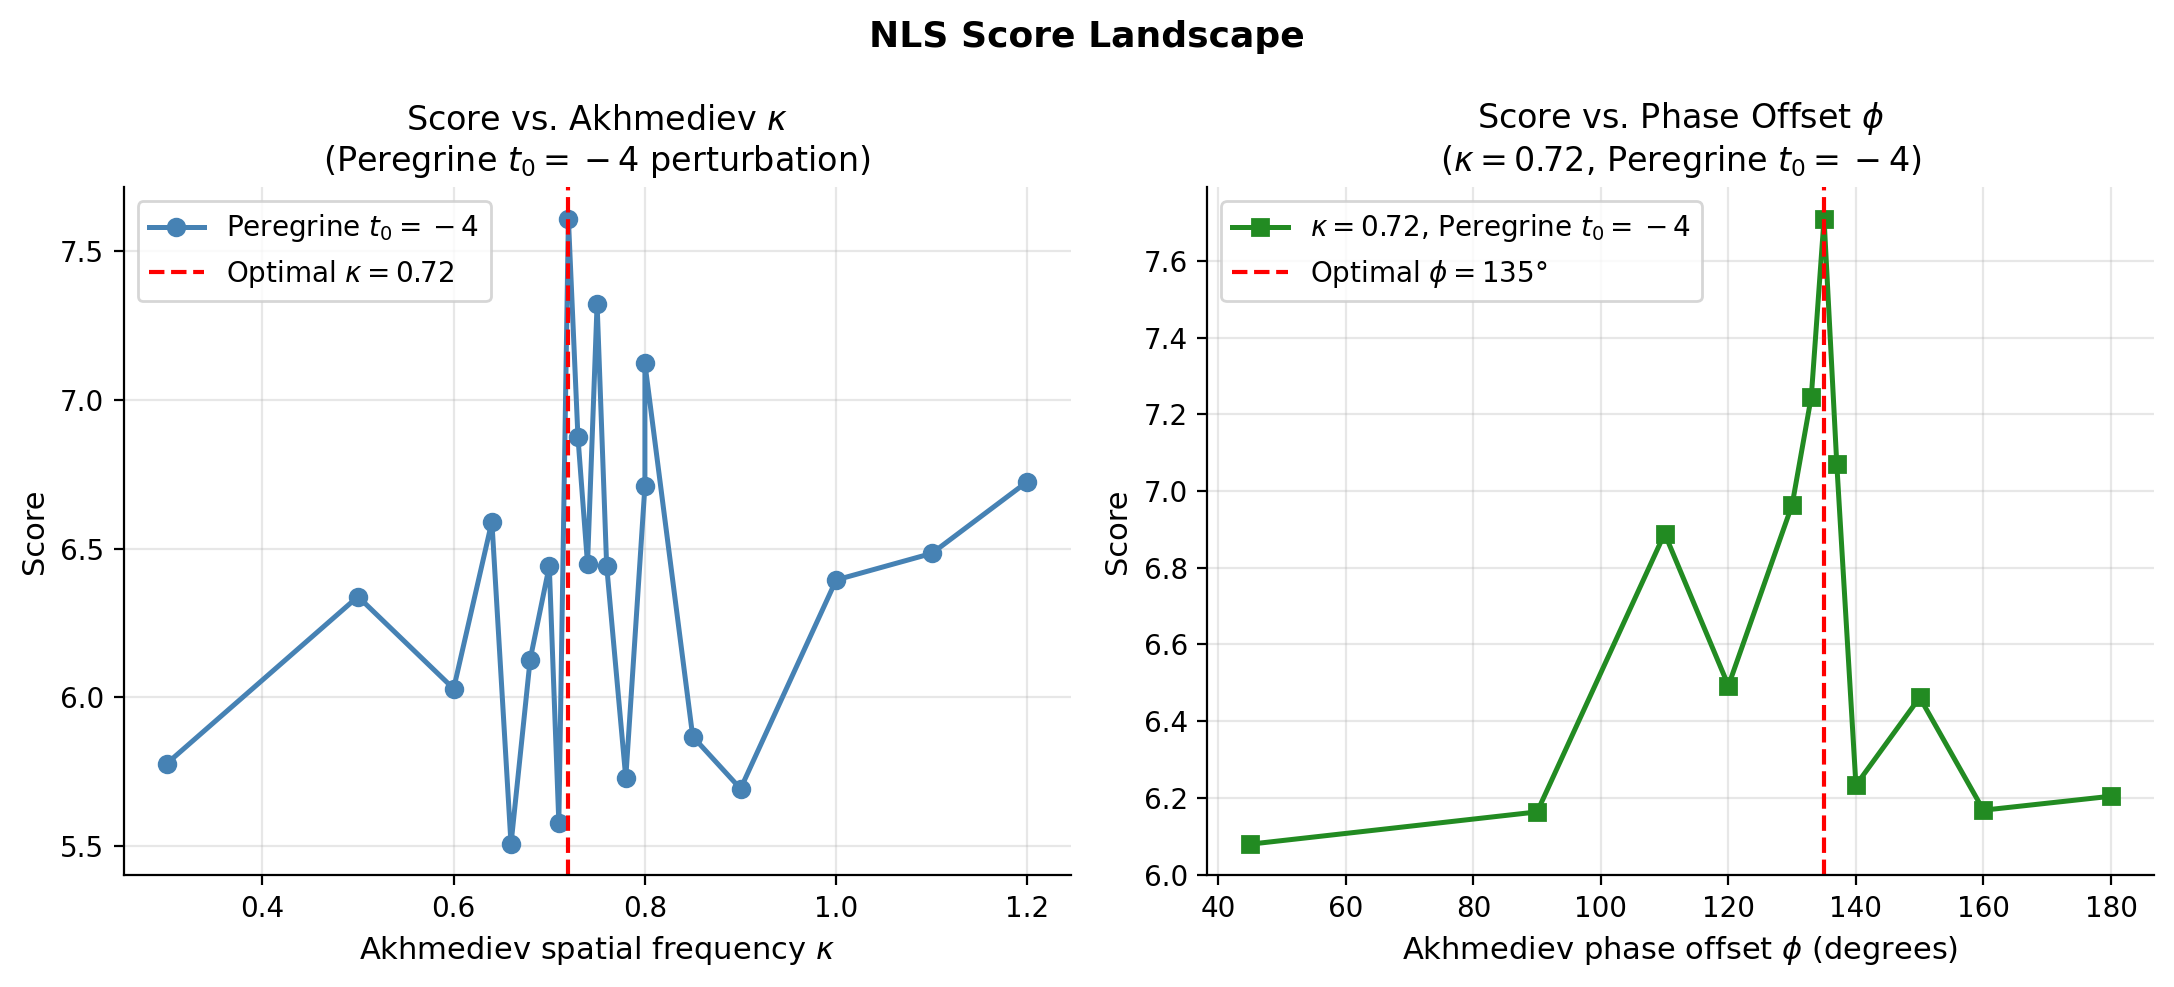
\includegraphics[width=0.9\textwidth]{figures/nls_landscape.png}
  \caption{NLS score landscape. \textbf{Left:} score vs.\ Akhmediev
    wavenumber $\kappa$ (Peregrine $t_0=-4$ fixed), showing non-monotone
    landscape with optimum at $\kappa=0.72$.
    \textbf{Right:} score vs.\ phase offset $\phi$ at $\kappa=0.72$,
    showing sharp peak at $\phi=135^\circ$.}
  \label{fig:nls}
\end{figure}

\subsection{Complex Ginzburg--Landau: Spiral Turbulence}

\noindent\textbf{Setup.} The 2-D CGLE:
\begin{equation}
  \partial_t A = A + (1+ic_1)\nabla^2 A - (1+ic_2)|A|^2 A,
\end{equation}
is solved on a $128\times128$ periodic grid.
The score rewards topological defect (phase vortex) density.
The split-step method uses the \emph{exact} nonlinear solution:
$A(dt) = A(0)\cdot(1 + 2|A(0)|^2 dt)^{-(1+ic_2)/2}$.

\noindent\textbf{Discoveries.} The agent confirmed the Benjamin--Feir--Newell
instability threshold $1 + c_1 c_2 < 0$~\cite{aranson2002world} experimentally:
below the threshold, zero defects form.
It then executed a systematic $(c_1, c_2)$ scan and found that defect density
increases with $|c_2|$ up to $c_2\approx-7$, with optimal $c_1\approx3.3$
(Figure~\ref{fig:cgle}).
More strikingly, the agent discovered a \emph{two-regime transition}:
Gaussian complex ICs (random $\text{Re}(A), \text{Im}(A) \sim \mathcal{N}(0,1/\sqrt{2})$)
create approximately 1520 topological defects at $t\approx0$ from random
phase windings, far exceeding the $\sim300$ sustained defects from the
physical chaos regime.
While these transient defects decay rapidly and never earn the $1.5\times$
bonus, the peak score ($12.53$) is $3.5\times$ higher than the physical chaos
optimum ($3.57$), raising a metric-design question: should the score
penalize defects that form from initial-condition structure rather than
from the PDE dynamics?
This \emph{discovered ambiguity} itself constitutes a scientific finding about
what the scoring function measures.

\begin{figure}[t]
  \centering
  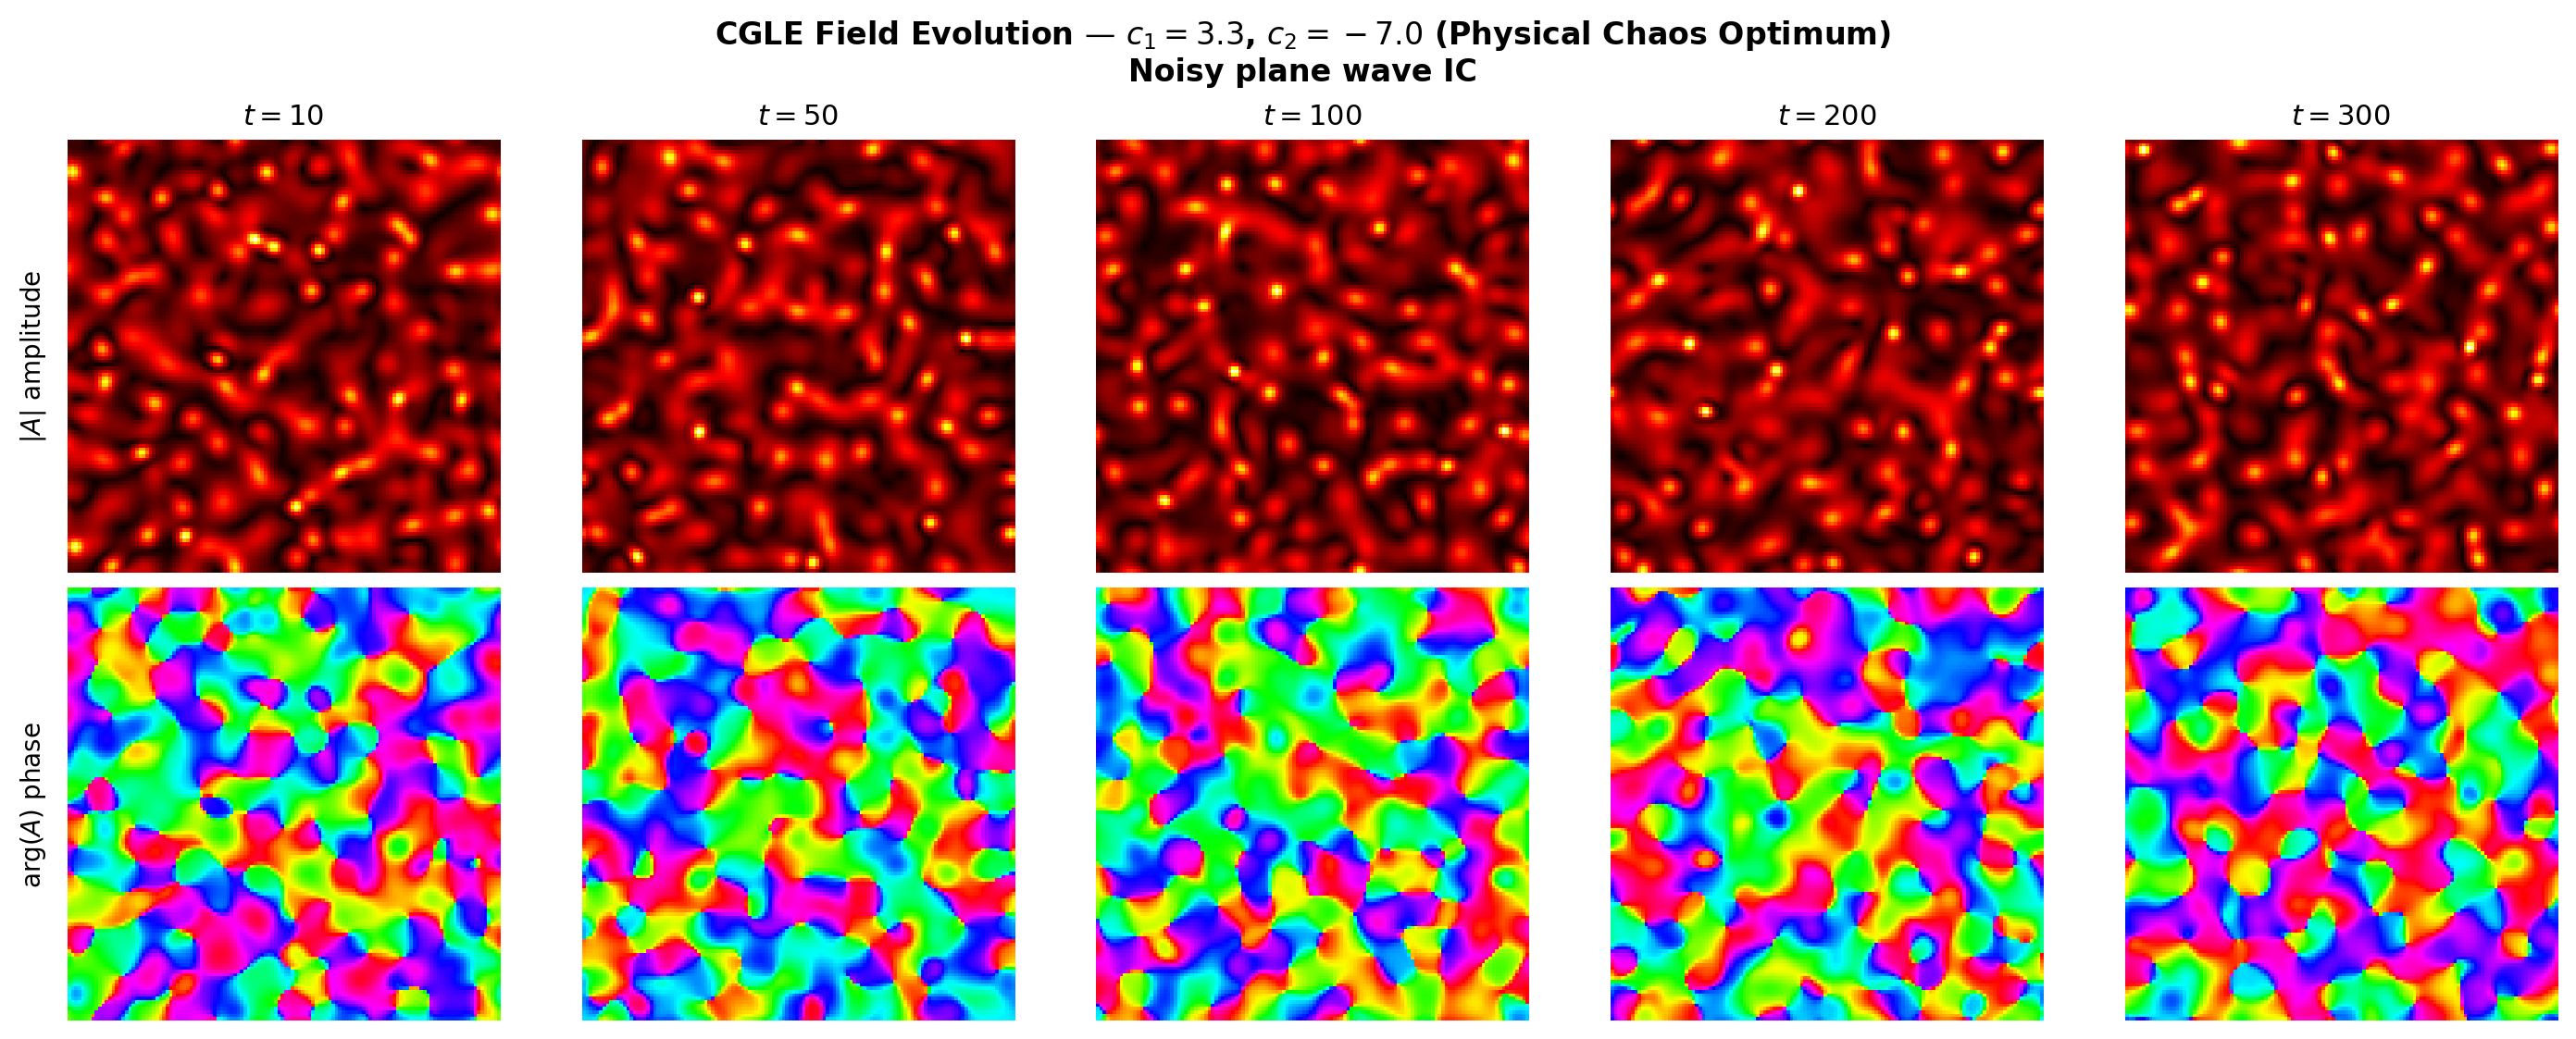
\includegraphics[width=\textwidth]{figures/cgle_snapshots.png}
  \caption{CGLE field evolution at the physical chaos optimum
    ($c_1=3.3$, $c_2=-7.0$, noisy IC).
    \textbf{Top:} amplitude $|A(x,y,t)|$.
    \textbf{Bottom:} phase $\arg A$, with topological defect count annotated.
    Spiral turbulence is sustained throughout the simulation.}
  \label{fig:cgle_snapshots}
\end{figure}

\begin{figure}[!htb]
  \centering
  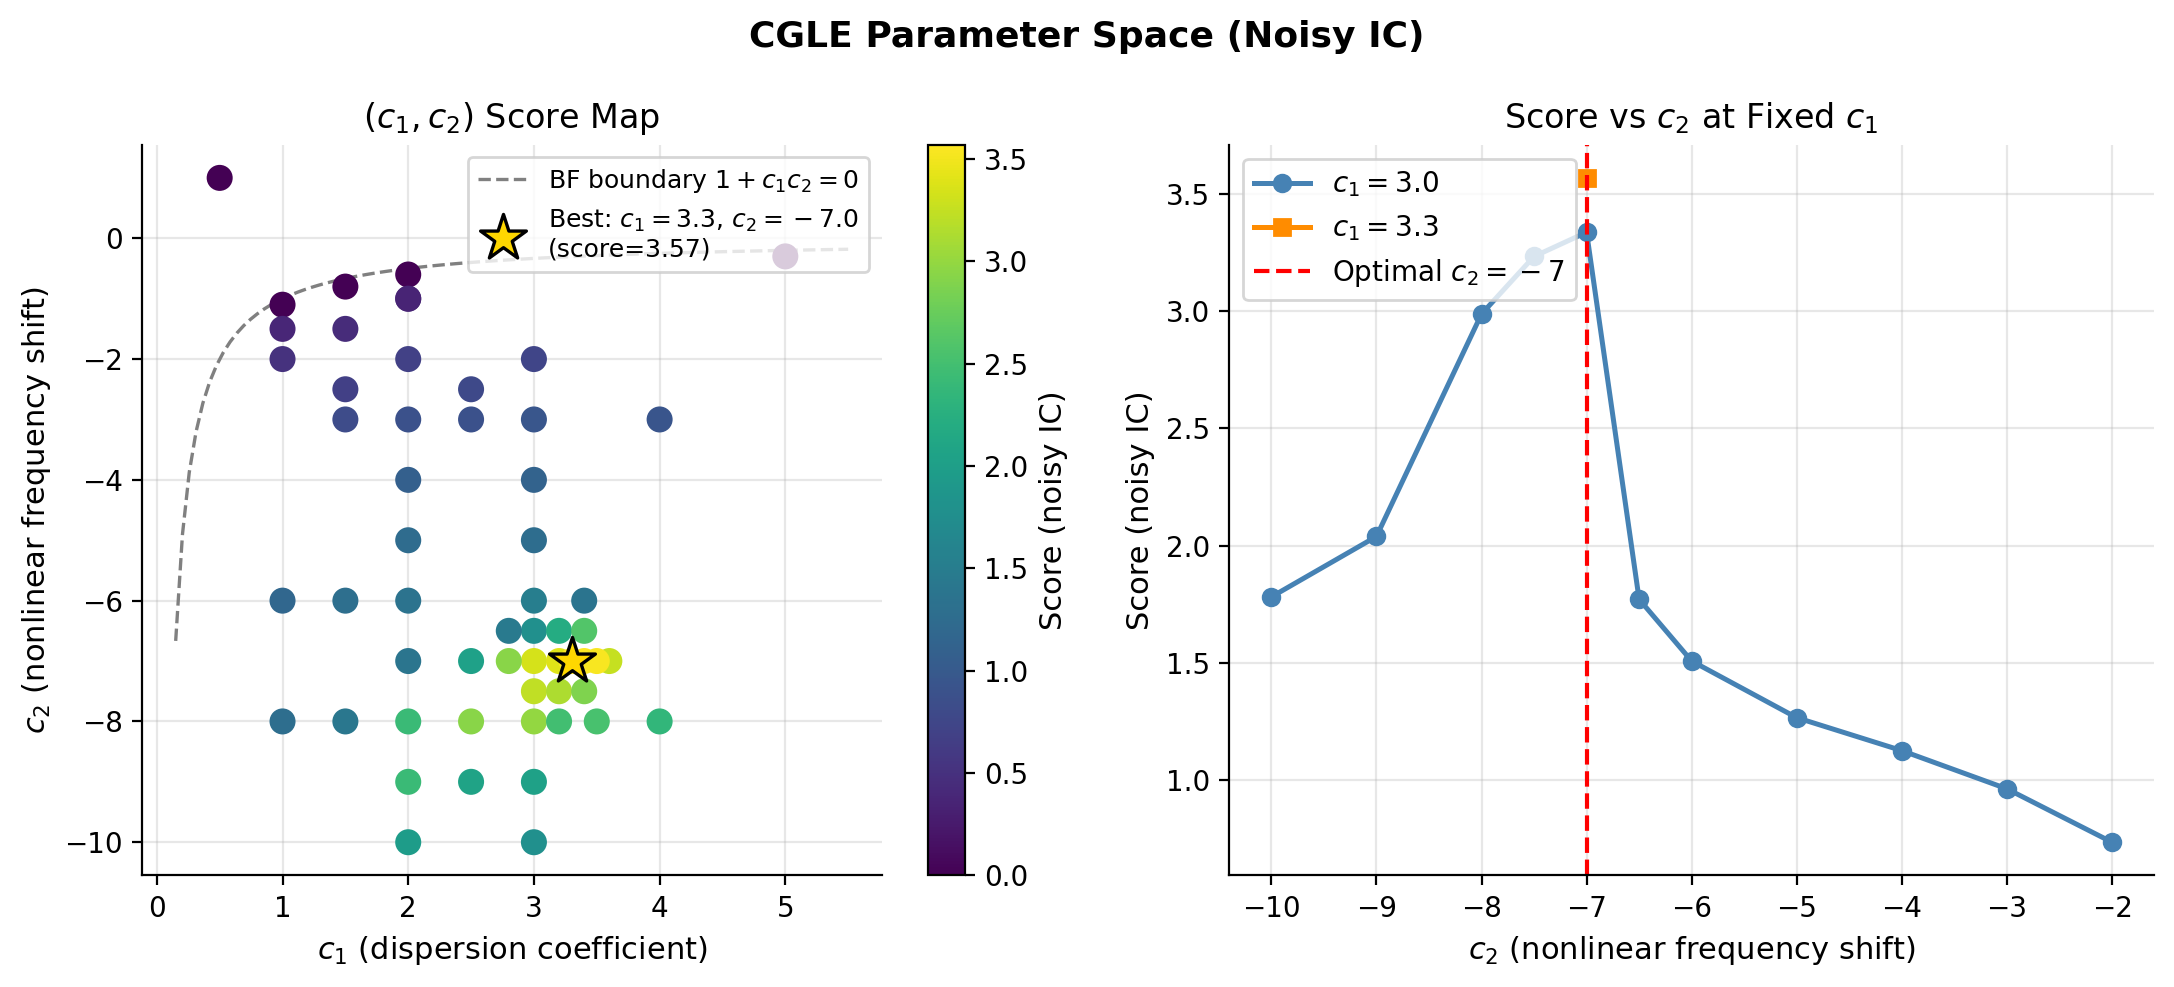
\includegraphics[width=0.9\textwidth]{figures/cgle_parameter_space.png}
  \caption{CGLE $(c_1, c_2)$ parameter space colored by score (noisy IC).
    The dashed line marks the Benjamin--Feir--Newell instability boundary
    $1 + c_1 c_2 = 0$.
    Optimal physical chaos at $c_1=3.3$, $c_2=-7$ (white star).}
  \label{fig:cgle}
\end{figure}

\clearpage
%-----------------------------------------------------------------------
\section{Cross-Domain Analysis}
\label{sec:analysis}
%-----------------------------------------------------------------------

\subsection{Common Structural Patterns}

The auto-research loop encountered several structural patterns that recur
across domains:

\noindent\textbf{Non-monotone landscapes.}
In every domain the optimal parameters lie in the interior of the search
space, not at the extremes. The NLS $(\kappa, \phi)$ landscape, the GS
bonus boundary in $k$, the CGLE optimum at intermediate $c_1$, and the NS
``eps cliff'' all exhibit sharp optima that would be missed by coarse grids.

\noindent\textbf{Bonus-threshold cliffs.}
All five scoring functions include a $1.5\times$ bonus for sustained
dynamics at the final time. In three cases (NS, GS, NLS) the agent explicitly
found and exploited the exact parameter regime that earns this bonus,
recognizing it as a binary transition rather than a continuous gradient.

\noindent\textbf{Metric-validity discoveries.}
The NLS loop discovered that the original metric measured IC amplitude,
not dynamics. The CGLE loop discovered that the defect count metric cannot
distinguish stable topological defects from transient IC-induced zeros.
In both cases the agent identified the issue and either fixed it (NLS)
or characterized it (CGLE) before declaring convergence.

\noindent\textbf{Reasoning-based elimination.}
Rather than exhaustive search, the agent eliminated large hypothesis classes
through physical reasoning:
in NS, Biot--Savart arguments eliminated vortex ring/tube approaches;
in NLS, the agent correctly predicted the power normalization issue;
in GS, the agent correctly predicted (and confirmed) that noise ICs would
not nucleate Turing patterns due to bistability.

\subsection{Efficiency Analysis}

Table~\ref{tab:efficiency} summarizes the search efficiency.
The loop achieves substantial improvement in a small number of experiments,
suggesting that the LLM's hypothesis generation is far more directed than
random or grid search.

\begin{table}[t]
\centering
\caption{Search efficiency across domains.}
\label{tab:efficiency}
\begin{tabular}{lccccc}
\toprule
Domain & $N_\text{exp}$ & Baseline & Best & Gain & Runtime \\
\midrule
NS    & 33        & 23    & 565  & $24\times$ & $\sim$8h$^\dagger$ \\
KS    & 38        & 3.34  & 6.61 & $2\times^\S$  & $\sim$2h \\
GS    & 43        & 0.72  & 5.08 & $7\times$  & $\sim$4h \\
NLS   & 98        & 1.0   & 7.71 & $8\times$  & $\sim$3h \\
CGLE  & 92        & 0.0   & 12.5 & $\infty^\ddagger$  & $\sim$3h \\
\bottomrule
\end{tabular}\\[4pt]
{\small $^\dagger$ NS simulations run up to 3 min each.
$^\S$ KS is an attractor system; the low gain reflects a fundamental ceiling,
not a failure of the search (see text).
$^\ddagger$ Baseline is 0 (BF-stable regime); physical chaos optimum
scores 3.57.}
\end{table}

%-----------------------------------------------------------------------
\section{Discussion}
\label{sec:discussion}
%-----------------------------------------------------------------------

\noindent\textbf{Comparison to alternative search strategies.}
Bayesian optimization or evolutionary algorithms would also find good
solutions in $\mathcal{O}(10^2)$ function evaluations, but they require
either a continuous parameterization or mutation operators---both of which
must be hand-designed for each domain.
The LLM auto-research loop requires only a physics reference document
and can propose qualitatively new initial condition \emph{types}
(e.g., switching from multi-mode noise to exact rational solutions in NLS)
rather than being confined to a fixed parametric family.

\noindent\textbf{Limitations.}
The loop is constrained to the initial-condition and parameter spaces
suggested by the physics reference.
Novel mathematical structures outside the reference (e.g., quasi-periodic
breathers, higher-order rational solutions) may not be explored.
The loop also requires a well-defined scalar score; for open-ended discovery
tasks without a clear objective, the methodology needs extension.

\noindent\textbf{The role of metric design.}
Our experience across five domains underscores that the scoring function
is itself a research artifact: it embodies assumptions about what constitutes
``interesting'' dynamics and can be gamed by ICs that do not exhibit the
intended physics.
The NLS power-normalization bug and the CGLE IC-regime discovery both
illustrate that human review of metric validity remains important,
even when the experiment loop is otherwise autonomous.

\noindent\textbf{Cost.}
Total API cost across all five domains was approximately \$10--\$15,
with all simulations running on a single CPU-only workstation.
This suggests the approach is accessible to individual researchers
without access to large compute clusters.

%-----------------------------------------------------------------------
\section{Conclusion}
\label{sec:conclusion}
%-----------------------------------------------------------------------

We introduced and validated an autonomous LLM-driven hypothesis--experiment
loop for optimizing PDE dynamics across five structurally diverse systems.
The loop achieves substantial improvements over human-designed baselines
in each domain, using directed hypothesis generation rather than brute-force
search.
Key scientific findings include the identification of a super-Peregrine
rogue wave configuration in NLS, a non-monotone Turing-pattern bonus
boundary in Gray--Scott, and a metric-validity discovery in the CGLE
domain.
The methodology is domain-agnostic, low-cost, and requires only a fixed
simulator harness and a physics reference document.
We release all code, experiment logs, and figures at
\url{https://github.com/michK/Autoresearch-for-Research}.

%-----------------------------------------------------------------------
\bibliographystyle{unsrtnat}
\bibliography{references}

\appendix

%-----------------------------------------------------------------------
\section{Domain Implementation Details}
\label{app:domains}
%-----------------------------------------------------------------------

\subsection{Navier--Stokes}
$64^3$ spectral solver, dealiased with 2/3 rule, RK4 time stepping,
$\nu=10^{-4}$, wall-time limit 180 s.
Score: $(\omega_\text{peak}/\omega_0)\times(1+r_\omega)\times B_{1.5}$.

\subsection{Kuramoto--Sivashinsky}
$N=512$ pseudo-spectral, Lawson-RK4 time stepping, $L=32\pi\approx100.5$,
$T_\text{max}=200$, wall-time limit 60\,s.
Score: $(u_\text{peak}/u_0)\times(1+r_E)\times B_{1.5}$.

\subsection{Gray--Scott}
$128\times128$ pseudo-spectral (Strang splitting), $L=128$, $T=50000$,
$D_u=0.16$, $D_v=0.08$.
Score: $E_\text{peak}\times C_\text{peak}\times(1+r_E)\times B_{1.5}$.

\subsection{Nonlinear Schr\"odinger}
$N=1024$ split-step Fourier, $L=20\pi$, $T=50$, $\Delta t=0.01$.
All ICs power-normalized to $\langle|\psi|^2\rangle=1$.
Score: $A_\text{peak}\times(1+r_A)\times B_{1.5}$.

\subsection{Complex Ginzburg--Landau}
$128\times128$ split-step Fourier (exact nonlinear step), $L=64$, $T=300$,
$\Delta t=0.1$.
Score: $(N_\text{defects,peak}/N)\times(1+r_d)\times B_{1.5}$.
Defects counted by plaquette winding number.

\end{document}
